%&./out/hands-on-ml_section1-1st-half_20210317
% use precompiled file
%%%%%%%%%% ↑ EDIT FILE NAME ↑ %%%%%%%%%%

% @file           hands-on-ml_section1-1st-half_20210317.tex
% @brief          Template slides of beamer (LaTeX)
% @author         Kataoka Nagi
% @date           2021-03-17 03:35:49
% $Version:       1.0
% @par            History
%                 New file
% Copyright (c) 2021 Kataoka Nagi
% - This src is released under the MIT License, see LICENSE.
%
%
% \documentclass[dvipdfmx, 11pt]{beamer}^
% aspectratio = 43, 149, 169
% font size = 8pt, 9pt, 10pt, 11pt, 12pt, 14pt, 17pt, 20pt
% @see 「Beamer columns 環境で画像を配置するベストな方法」https://qiita.com/t_uda/items/8ef173eebf9827305135#3-columns-%E7%92%B0%E5%A2%83%E3%81%AE%E6%AD%A3%E3%81%97%E3%81%84%E4%BD%BF%E3%81%84%E6%96%B9
\PassOptionsToClass{hiresbb}{graphicx}
\documentclass[aspectratio=169, dvipdfmx, 14pt, xcolor={svgnames,dvipsnames}]{beamer}
\usepackage{graphicx}
\newcommand{\thickhrulefill}{\leavevmode\leaders\hrule depth-1.2pt height 3.2pt\hfill\kern0pt}
\newcommand{\indicatewidth}[1]{\thickhrulefill{#1}\thickhrulefill}
\newlength{\mytotalwidth}
\mytotalwidth=\dimexpr\linewidth-5mm
\newlength{\mycolumnwidth}
\mycolumnwidth=\dimexpr\mytotalwidth-5mm

\usepackage{base_kataoka-nagi}
\usepackage{slides_kataoka-nagi}
% \usepackage{../styles/base_kataoka-nagi/base_kataoka-nagi} % debug
% \usepackage{../styles/slides_kataoka-nagi/slides_kataoka-nagi} % debug

% precompile preamble from here. don't precompile with glossaries-env!
% type [eptex -ini -jobname="FILE_NAME" "&platex" mylatexformat.ltx FILE_NAME.tex] in cd
% @see 「beamerのコンパイル速度を上げる」 http://margaret-sdpara.blogspot.com/2019/11/beamer.html
\endofdump

\def\tightlist{\itemsep1pt\parskip0pt\parsep0pt}
% \includeonlyframes{current} % current build \begin{frame}[label=current]

% \usepackage{enumitem}
% \setlistdepth{10}
% \renewlist{itemize}{itemize}{10}
\setbeamertemplate{itemize subsubitem}{\tiny\raise2pt\hbox{■}}

\title[実践機械学習 輪読会 第1章 前半]{scikit-learn、Keras、TensorFlowによる\\実践機械学習 第2版\\第1章 前半}
\subtitle{データ工学研究室 輪読会}
\author[片岡 凪]{AL18036 片岡 凪}
% \institute[SIT]{芝浦工業大学 工学部 情報工学科 4年}
\institute[データ工学研究室 B3]{芝浦工業大学 工学部 情報工学科 3年}
\date{March 17, 2021}

\begin{document}

%%%%%%%%%%%%%%%%%%%%%%%%%%%%%%%%%%%%%%%%%%%%%%%%%%

\maketitle

%%%%%%%%%%%%%%%%%%%%%%%%%%%%%%%%%%%%%%%%%%%%%%%%%%

% \begin{frame}[label=current]{\quad 発表者}
\begin{frame}{\quad 発表者紹介}
  \begin{columns}[totalwidth=\mytotalwidth]
    \begin{column}[t]{0.8\mycolumnwidth}
      \begin{itemize}
        \item 片岡 凪
        \item 千葉県 浦安市
        \item 芝浦工業大学 工学部 情報工学科 3年
        \item データ工学研究室(木村昌臣研究室)
        \item 関心:画像,XAI,自動化,効率化
        \item Twitter @calm\_IRL
        \item Github  KataokaNagi
      \end{itemize}
    \end{column}
    \begin{column}[T]{0.2\mycolumnwidth}
      \centering
      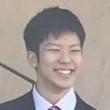
\includegraphics[width=80pt]{img/icon.jpg}
    \end{column}
  \end{columns}
\end{frame}

%%%%%%%%%%%%%%%%%%%%%%%%%%%%%%%%%%%%%%%%%%%%%%%%%%

% index
\begin{frame}{目次}
  \tableofcontents
\end{frame}

% \begin{frame}{ブロック環境}
%   \begin{block}{block}
%     block
%   \end{block}
%   \begin{alertblock}{alertblock}
%     alertblock
%   \end{alertblock}
%   \begin{exampleblock}{exampleblock}
%     exampleblock
%   \end{exampleblock}
%   \begin{tcolorbox}[colframe=green,
%       colback=green!10!white,
%       colbacktitle=green!40!white,
%       coltitle=black, fonttitle=\bfseries,
%       title=My box]
%     box contents
%   \end{tcolorbox}
% \end{frame}

%%%%%%%%%%%%%%%%%%%%%%%%%%%%%%%%%%%%%%%%%%%%%%%%%%

\section{はじめに}
\begin{frame}{目次}
  \tableofcontents[currentsection]
\end{frame}

%%%%%%%%%%%%%%%%%%%%%%%%%%%%%%%%%%%%%%%%%%%%%%%%%%

\begin{frame}{使用ソフト}
  \begin{itemize}
    \tightlist
    \item
          scikit-learn

          \begin{itemize}
            \tightlist
            \item
                  多くの効率的なアルゴリズム
          \end{itemize}
    \item
          TensorFlow

          \begin{itemize}
            \tightlist
            \item
                  GPUによる分散NNエンジン
            \item
                  Google
          \end{itemize}
    \item
          Keras

          \begin{itemize}
            \tightlist
            \item
                  NNの単純化API
            \item
                  TensorFlowなどと利用
          \end{itemize}
  \end{itemize}
\end{frame}

%%%%%%%%%%%%%%%%%%%%%%%%%%%%%%%%%%%%%%%%%%%%%%%%%%
\begin{frame}{必要な予備知識}
  \begin{itemize}
    \tightlist
    \item
          Python

          \begin{itemize}
            \tightlist
            \item
                  Numpy
            \item
                  Pandas
            \item
                  Matplotlib
          \end{itemize}
    \item
          数学

          \begin{itemize}
            \tightlist
            \item
                  解析学
            \item
                  線形代数
            \item
                  確率論
            \item
                  統計学
          \end{itemize}
  \end{itemize}
\end{frame}

%%%%%%%%%%%%%%%%%%%%%%%%%%%%%%%%%%%%%%%%%%%%%%%%%%
\begin{frame}{おすすめ教材}
  \begin{itemize}
    \tightlist
    \item
          Pythonチュートリアル

          \begin{itemize}
            \tightlist
            \item
                  \href{https://www.learnpython.org/}{LearnPython}
            \item
                  \href{https://docs.python.org/3/tutorial/}{python.org}
          \end{itemize}
    \item
          機械学習

          \begin{itemize}
            \tightlist
            \item
                  \href{https://www.coursera.org/learn/machine-learning}{Cousera -
                    Andrew Ng 機械学習講座}

                  \begin{itemize}
                    \tightlist
                    \item
                          数か月かかる
                  \end{itemize}
            \item
                  \href{https://scikit-learn.org/skdoc}{scikit-learn ユーザーガイド}
            \item
                  \href{https://www.dataquest.io/}{Dataquest}

                  \begin{itemize}
                    \tightlist
                    \item
                          対話的教材
                  \end{itemize}
            \item
                  \href{https://jp.quora.com/search?q=Machine\%20Learning}{Quora}

                  \begin{itemize}
                    \tightlist
                    \item
                          Q\&Aサイト
                  \end{itemize}
            \item
                  \href{https://sites.google.com/site/minggaoshomepage/links/dee}{deeplearning.net}
          \end{itemize}
  \end{itemize}
\end{frame}

%%%%%%%%%%%%%%%%%%%%%%%%%%%%%%%%%%%%%%%%%%%%%%%%%%
\begin{frame}{配布コード}
  \begin{itemize}
    \tightlist
    \item
          Jyoyterノートブック
    \item
          https://github.com/ageron/handson-ml2
  \end{itemize}
\end{frame}

%%%%%%%%%%%%%%%%%%%%%%%%%%%%%%%%%%%%%%%%%%%%%%%%%%

\section{1
  機械学習の現状}\label{ux6a5fux68b0ux5b66ux7fd2ux306eux73feux72b6}

\begin{frame}{目次}
  \tableofcontents[currentsection]
\end{frame}

%%%%%%%%%%%%%%%%%%%%%%%%%%%%%%%%%%%%%%%%%%%%%%%%%%

\begin{frame}
  \frametitle{第1章の目的}

  \begin{itemize}
    \tightlist
    \item
          MLの対象や意味範囲
    \item
          MLの例

          \begin{itemize}
            \tightlist
            \item
                  スパムフィルタ
            \item
                  OCR
            \item
                  商品提案
            \item
                  音声検索
          \end{itemize}
  \end{itemize}
\end{frame}

%%%%%%%%%%%%%%%%%%%%%%%%%%%%%%%%%%%%%%%%%%%%%%%%%%

\subsection{1.1
  機械学習とは何か}\label{ux6a5fux68b0ux5b66ux7fd2ux3068ux306fux4f55ux304b}

\begin{frame}{目次}
  \tableofcontents[currentsubsection]
\end{frame}

%%%%%%%%%%%%%%%%%%%%%%%%%%%%%%%%%%%%%%%%%%%%%%%%%%

\begin{frame}
  \frametitle{{MLの意味}}
  \begin{itemize}
    \tightlist
    \item
          コンピュータがデータから学習するための科学技術

          \begin{itemize}
            \tightlist
            \item
                  学習:タスクの測定指標が向上する経験を得ること
          \end{itemize}
    \item
          各種語義

          \begin{itemize}
            \tightlist
            \item
                  訓練セット

                  \begin{itemize}
                    \tightlist
                    \item
                          学習用のデータ例
                  \end{itemize}
            \item
                  訓練インスタンス,標本

                  \begin{itemize}
                    \tightlist
                    \item
                          個々のデータ例
                  \end{itemize}
            \item
                  訓練データ

                  \begin{itemize}
                    \tightlist
                    \item
                          経験
                  \end{itemize}
            \item
                  正解率

                  \begin{itemize}
                    \tightlist
                    \item
                          性能指標
                  \end{itemize}
          \end{itemize}
  \end{itemize}
\end{frame}

%%%%%%%%%%%%%%%%%%%%%%%%%%%%%%%%%%%%%%%%%%%%%%%%%%

\subsection{1.2
  なぜ機械学習を使うのか}\label{ux306aux305cux6a5fux68b0ux5b66ux7fd2ux3092ux4f7fux3046ux306eux304b}

\begin{frame}{目次}
  \tableofcontents[currentsubsection]
\end{frame}

%%%%%%%%%%%%%%%%%%%%%%%%%%%%%%%%%%%%%%%%%%%%%%%%%%

\begin{frame}
  \frametitle{MLの概要}
  \begin{itemize}
    \tightlist
    \item
          MLの手順

          \begin{enumerate}
            \def\labelenumi{\arabic{enumi}.}
            \tightlist
            \item
                  一般的な特徴を分析
            \item
                  特徴をもとに検出アルゴリズムを作成
            \item
                  プログラムをテストし、実用レベルになるまで上を繰り返す
          \end{enumerate}
    \item
          MLの利点

          \begin{itemize}
            \tightlist
            \item
                  データごとのアルゴリズムが不要
            \item
                  複雑な問題の解決
            \item
                  既知のアルゴリズムがない問題の解決
            \item
                  データマイニング

                  \begin{itemize}
                    \tightlist
                    \item
                          特徴の予想外な相関関係,トレンドの発見

                    \item
                          高速に
                  \end{itemize}
          \end{itemize}
  \end{itemize}
\end{frame}

% %%%%%%%%%%%%%%%%%%%%%%%%%%%%%%%%%%%%%%%%%%%%%%%%%%

\subsection{1.3 応用の例}\label{ux5fdcux7528ux306eux4f8b}
\begin{frame}{目次}
  \tableofcontents[currentsubsection]
\end{frame}

%%%%%%%%%%%%%%%%%%%%%%%%%%%%%%%%%%%%%%%%%%%%%%%%%%

\begin{frame}
  \frametitle{MLの例 1/6}
  \begin{itemize}
    \tightlist
    \item
          製品の自動分類

          \begin{itemize}
            \tightlist
            \item
                  イメージ分類

                  \begin{itemize}
                    \tightlist
                    \item
                          CNN(Convolutional:畳み込み)などを利用
                  \end{itemize}
          \end{itemize}
    \item
          脳腫瘍の検出

          \begin{itemize}
            \tightlist
            \item
                  セマンティックセグメンテーション

                  \begin{itemize}
                    \tightlist
                    \item
                          CNNなど
                  \end{itemize}
          \end{itemize}
    \item
          記事の自動分類

          \begin{itemize}
            \tightlist
            \item
                  テキスト分類 ∈ NLP(自然言語処理)

                  \begin{itemize}
                    \tightlist
                    \item
                          RNN(Recurrent:再帰型)
                    \item
                          CNN
                    \item
                          Transformer
                  \end{itemize}
          \end{itemize}
  \end{itemize}
\end{frame}

%%%%%%%%%%%%%%%%%%%%%%%%%%%%%%%%%%%%%%%%%%%%%%%%%%

\begin{frame}
  \frametitle{MLの例 2/6}
  \begin{itemize}
    \item
          不適切発言へのフラグ付加

          \begin{itemize}
            \tightlist
            \item
                  テキスト分類
          \end{itemize}
    \item
          自動要約

          \begin{itemize}
            \tightlist
            \item
                  テキスト自動要約 ∈ NLP
          \end{itemize}
    \item
          チャットボット、パーソナルアシスタント

          \begin{itemize}
            \tightlist
            \item
                  NLU(自然言語理解)
            \item
                  Q\&Aモジュール
          \end{itemize}
  \end{itemize}
\end{frame}

%%%%%%%%%%%%%%%%%%%%%%%%%%%%%%%%%%%%%%%%%%%%%%%%%%

\begin{frame}
  \frametitle{MLの例 3/6}
  \begin{itemize}
    \item
          次年度収益の予測

          \begin{itemize}
            \tightlist
            \item
                  回帰タスク(値の予測)

                  \begin{itemize}
                    \tightlist
                    \item
                          線形回帰
                    \item
                          多項式回帰モデル
                    \item
                          SVM回帰
                    \item
                          ランダムフォレスト回帰
                    \item
                          人工NN
                  \end{itemize}
            \item
                  過去の業績指標の利用

                  \begin{itemize}
                    \tightlist
                    \item
                          RNN
                    \item
                          CNN
                    \item
                          Transformer
                  \end{itemize}
          \end{itemize}
  \end{itemize}
\end{frame}

%%%%%%%%%%%%%%%%%%%%%%%%%%%%%%%%%%%%%%%%%%%%%%%%%%

\begin{frame}
  \frametitle{MLの例 4/6}
  \begin{itemize}
    \item
          音声コマンド

          \begin{itemize}
            \tightlist
            \item
                  オーディオサンプルの処理

                  \begin{itemize}
                    \tightlist
                    \item
                          長くて複雑

                          % \begin{itemize}
                          % \tightlist
                    \item
                          RNN
                    \item
                          CNN
                    \item
                          Transformer
                          % \end{itemize}
                  \end{itemize}
          \end{itemize}
    \item
          クレカ詐欺の検知

          \begin{itemize}
            \tightlist
            \item
                  異常検知
          \end{itemize}
  \end{itemize}

\end{frame}

%%%%%%%%%%%%%%%%%%%%%%%%%%%%%%%%%%%%%%%%%%%%%%%%%%

\begin{frame}
  \frametitle{MLの例 5/6}
  \begin{itemize}
    \item
          購入履歴による顧客分類、販売戦略

          \begin{itemize}
            \tightlist
            \item
                  クラスタリング
          \end{itemize}
    \item
          高次元データセットの図示

          \begin{itemize}
            \tightlist
            \item
                  データの可視化
            \item
                  次元削除
          \end{itemize}
    \item
          購入履歴から商品提案

          \begin{itemize}
            \tightlist
            \item
                  推薦システム

                  \begin{itemize}
                    \tightlist
                    \item
                          人工NNなど
                  \end{itemize}
          \end{itemize}
  \end{itemize}
\end{frame}

%%%%%%%%%%%%%%%%%%%%%%%%%%%%%%%%%%%%%%%%%%%%%%%%%%

\begin{frame}
  \frametitle{MLの例 6/6}
  \begin{itemize}
    \item
          ゲームのインテリジェントボット

          \begin{itemize}
            \tightlist
            \item
                  アクションの選択

                  \begin{itemize}
                    \tightlist
                    \item
                          RL(Reinforced L:強化学習)

                          % \begin{itemize}
                          \tightlist
                    \item
                          全時間の報酬の最大化
                    \item
                          AlphaGo
                          % \end{itemize}
                  \end{itemize}
          \end{itemize}
  \end{itemize}
\end{frame}

%%%%%%%%%%%%%%%%%%%%%%%%%%%%%%%%%%%%%%%%%%%%%%%%%%

% \begin{frame}
%   \frametitle{MLの例 Appendix 画像系 by 加瀬先輩}
%   \begin{itemize}
%     \tightlist
%     \item
%           CNNs:

%           \begin{itemize}
%             \tightlist
%             \item
%                   Convolutional Neural
%                   Networks、種類)AlexNet、VGG16、ResNet、GoogLeNet
%           \end{itemize}
%     \item
%           Feature:

%           \begin{itemize}
%             \tightlist
%             \item
%                   特徴、CNNの抽出層で返還されたデータのことや、画像に内在するパターンのこと
%                   類)Feature map
%           \end{itemize}
%     \item
%           Image Classification:

%           \begin{itemize}
%             \tightlist
%             \item
%                   画像分類タスク.
%           \end{itemize}
%     \item
%           Image Recognition:

%           \begin{itemize}
%             \tightlist
%             \item
%                   画像認識タスク、Detectionと似ているかも?どの範囲に物体が存在するか検知
%           \end{itemize}
%     \item
%           Image Generation:

%           \begin{itemize}
%             \tightlist
%             \item
%                   画像生成、類)GAN
%           \end{itemize}
%     \item
%           Image Segmentation:

%           \begin{itemize}
%             \tightlist
%             \item
%                   画像分割、あるルールに則ってパーツごとに分割するタスク
%           \end{itemize}
%     \item
%           MNIST:

%           \begin{itemize}
%             \tightlist
%             \item
%                   0\textasciitilde9の手書きの数字(白黒)データセット
%           \end{itemize}
%     \item
%           CIFAR10:

%           \begin{itemize}
%             \tightlist
%             \item
%                   一般物体認識用のデータセット、飛行機・船・自動車・トラック・猫・犬・蛙・馬・鳥・鹿の10クラス
%           \end{itemize}
%     \item
%           ImageNet:

%           \begin{itemize}
%             \tightlist
%             \item
%                   画像分類で評価に使用されるデータセット
%           \end{itemize}
%     \item
%           GAN:

%           \begin{itemize}
%             \tightlist
%             \item
%                   Generative Adversarial Networks、画像を生成するモデル.
%                   BLEACH風(KBTIT)の顔変換等のpaperは面白い.
%           \end{itemize}
%     \item
%           Adversarial Examples:

%           \begin{itemize}
%             \tightlist
%             \item
%                   敵対的サンプル、AIを騙す画像.
%           \end{itemize}
%     \item
%           XAI:

%           \begin{itemize}
%             \tightlist
%             \item
%                   説明可能AI、最近の流行り. モデルの予測根拠を可視化など.
%                   ex)SHAP、LIME、SmoothGrad、Guided-BackProp etc
%           \end{itemize}
%     \item
%           Robustness:

%           \begin{itemize}
%             \tightlist
%             \item
%                   頑健性、研究フィールドの文脈で意味合いが異なるが、ノイズなどの影響を受けずに正しく分類する性質
%           \end{itemize}
%     \item
%           Generalization:

%           \begin{itemize}
%             \tightlist
%             \item
%                   汎化、未知のデータに対しても正しく分類できる性質
%           \end{itemize}
%     \item
%           Data Distribution:

%           \begin{itemize}
%             \tightlist
%             \item
%                   データ分布(画像に限らず)、データセット1枚1枚で見た時に、青い鳥が多いとか、犬の背景は山が多いとか傾向
%           \end{itemize}
%     \item
%           Label annotation:

%           \begin{itemize}
%             \tightlist
%             \item
%                   画像に付与された正解ラベルは本当に適切か?(複数写っている場合はどうする
%                   etc)という問題に対応する学問
%           \end{itemize}
%     \item
%           Bouding Box:

%           \begin{itemize}
%             \tightlist
%             \item
%                   認識タスクで、物体が映り込んでいる領域のこと.
%                   物体に合わせて適切に囲むことが目的
%           \end{itemize}
%   \end{itemize}
% \end{frame}

% %%%%%%%%%%%%%%%%%%%%%%%%%%%%%%%%%%%%%%%%%%%%%%%%%%


\subsection{1.4
  機械学習システムのタイプ}\label{ux6a5fux68b0ux5b66ux7fd2ux30b7ux30b9ux30c6ux30e0ux306eux30bfux30a4ux30d7}
\begin{frame}{目次}
  \tableofcontents[currentsubsection]
\end{frame}

%%%%%%%%%%%%%%%%%%%%%%%%%%%%%%%%%%%%%%%%%%%%%%%%%%

\begin{frame}
  \frametitle{MLの分類 - 概要}
  \begin{itemize}
    \tightlist
    \item
          MLの分類

          \begin{itemize}
            \tightlist
            \item
                  人間の関与の有無

                  \begin{itemize}
                    \tightlist
                    \item
                          教師あり
                    \item
                          教師なし
                    \item
                          半教師あり
                    \item
                          強化学習
                  \end{itemize}
            \item
                  その場で少しずつ学習可能か

                  \begin{itemize}
                    \tightlist
                    \item
                          オンライン学習
                    \item
                          バッチ学習
                  \end{itemize}
            \item
                  既知のデータポイントから予測モデルを構築するか

                  \begin{itemize}
                    \tightlist
                    \item
                          インスタンスベース学習
                    \item
                          モデルベース学習
                  \end{itemize}
          \end{itemize}
    \item
          上記分類を組み合わせる
  \end{itemize}

\end{frame}

%%%%%%%%%%%%%%%%%%%%%%%%%%%%%%%%%%%%%%%%%%%%%%%%%%%

\begin{frame}
  \frametitle{1.4.1 教師あり学習 1/2}
  \begin{itemize}
    \tightlist
    \item
          訓練データに正解のラベル
    \item
          応用先

          \begin{itemize}
            \tightlist
            \item
                  クラス分類
            \item
                  回帰(regression)

                  \begin{itemize}
                    \tightlist
                    \item
                          予測子(predictor)(=一連の特徴量)からターゲットの数値を予測すること
                    \item
                          語源:背の高い両親の子供が平均に帰して背が低くなる傾向にあることを統計的に示した研究より
                    \item
                          出力が複数になる問題も
                  \end{itemize}
            \item
                  回帰に分類が使えるものも
            \item
                  分類に回帰が使えるものも

                  \begin{itemize}
                    \tightlist
                    \item
                          例:ロジスティック回帰で分類確率を導出
                  \end{itemize}
          \end{itemize}
  \end{itemize}
\end{frame}

%%%%%%%%%%%%%%%%%%%%%%%%%%%%%%%%%%%%%%%%%%%%%%%%%%%

\begin{frame}
  \frametitle{1.4.1 教師あり学習 2/2}
  \begin{itemize}
    \item
          代表的なアルゴリズム

          \begin{itemize}
            \tightlist
            \item
                  k近傍法
            \item
                  線形回帰
            \item
                  ロジスティック回帰
            \item
                  SVM
            \item
                  決定木,ランダムフォレスト
            \item
                  NN
          \end{itemize}
  \end{itemize}
\end{frame}

%%%%%%%%%%%%%%%%%%%%%%%%%%%%%%%%%%%%%%%%%%%%%%%%%%%

\begin{frame}
  \frametitle{1.4.1 教師なし学習 - 概要}
  \begin{itemize}
    \tightlist
    \item
          ラベルはない
    \item
          代表的なアルゴリズム
          \begin{itemize}
            \item クラスタリング
            \item 異常検知、新規性検知(anomaly detection, novelty detection)
            \item 可視化、次元削減(visualization, dimension reduction)
            \item 相関ルール学習(association rule learning)
          \end{itemize}
  \end{itemize}
\end{frame}

%%%%%%%%%%%%%%%%%%%%%%%%%%%%%%%%%%%%%%%%%%%%%%%%%%%

\begin{frame}
  \frametitle{1.4.1 教師なし学習 - クラスタリング}
  \begin{itemize}
    \tightlist
    \item
          k平均法
    \item
          DBSCAN
    \item
          階層的クラスタ分析(HCA:Hierarchial Clustering Analysis?)

          \begin{itemize}
            \tightlist
            \item
                  分類の粒度が可変
          \end{itemize}
  \end{itemize}
\end{frame}

%%%%%%%%%%%%%%%%%%%%%%%%%%%%%%%%%%%%%%%%%%%%%%%%%%%

\begin{frame}
  \frametitle{1.4.1 教師なし学習 - 異常検知、新規性検知}


  \begin{itemize}
    \tightlist
    \item
          異常検知

          \begin{itemize}
            \tightlist
            \item
                  正常なインスタンスで訓練
            \item
                  想定内の外れ値を検知
          \end{itemize}
    \item
          新規性検知

          \begin{itemize}
            \tightlist
            \item
                  ML以外のアルゴリズムで検知できない、分類済みだと思われるインスタンスで訓練
            \item
                  予想外の外れ値を検知
          \end{itemize}
    \item
          例

          \begin{itemize}
            \tightlist
            \item
                  1クラスSVM
            \item
                  アイソレーションフォレスト
          \end{itemize}
  \end{itemize}
\end{frame}

%%%%%%%%%%%%%%%%%%%%%%%%%%%%%%%%%%%%%%%%%%%%%%%%%%%

\begin{frame}
  \frametitle{1.4.1 教師なし学習 - 可視化、次元削減 1/2}
  \begin{itemize}
    \tightlist
    \item
          構造を保ちつつ、セマンティッククラスタを可視化

          \begin{itemize}
            \tightlist
            \item
                  片岡解釈:クラスタごとの座標などを保ちつつ、意味のある群の可視化用ラベル(次元)を増やす
            \item
                  可視化例:クラスタ同士の重なり具合
          \end{itemize}
    \item
          特徴量抽出(Feature Extraction)

          \begin{itemize}
            \tightlist
            \item
                  情報量を保ちつつ相関する複数の特徴をまとめ(次元圧縮)、データを見やすくする
            \item
                  種々のMLの前処理に利用

                  \begin{itemize}
                    \tightlist
                    \item
                          速度向上
                    \item
                          計算資源の節約
                    \item
                          性能が向上することも
                  \end{itemize}
          \end{itemize}
  \end{itemize}
\end{frame}

%%%%%%%%%%%%%%%%%%%%%%%%%%%%%%%%%%%%%%%%%%%%%%%%%%%

\begin{frame}
  \frametitle{1.4.1 教師なし学習 - 可視化、次元削減 2/2}
  \begin{itemize}
    \item
          例

          \begin{itemize}
            \tightlist
            \item
                  PCA(Principal Component Analysis:主成分分析)
            \item
                  カーネルPCA
            \item
                  LLE(Locally-Linear Embedding:局所線形埋め込み法)
            \item
                  t-SNE(t-distributed Stochastic Neighbor
                  Embedding:t分布確率的近傍埋め込み法)
          \end{itemize}
  \end{itemize}
\end{frame}

%%%%%%%%%%%%%%%%%%%%%%%%%%%%%%%%%%%%%%%%%%%%%%%%%%%

\begin{frame}
  \frametitle{1.4.1 教師なし学習 - 相関ルール学習}
  \begin{itemize}
    \tightlist
    \item
          大量のデータの属性同士の興味深い関係を導く

          \begin{itemize}
            \tightlist
            \item
                  例:オムツとビール
          \end{itemize}
    \item
          例

          \begin{itemize}
            \tightlist
            \item
                  ア・プリオリ
            \item
                  Eclat
          \end{itemize}
  \end{itemize}
\end{frame}

%%%%%%%%%%%%%%%%%%%%%%%%%%%%%%%%%%%%%%%%%%%%%%%%%%%

\begin{frame}
  \frametitle{1.4.1 半教師あり学習(semisupervised learning)}
  \begin{itemize}
    \tightlist
    \item
          一部にラベル
    \item
          ラベルの有無に応じた重みづけ?
    \item
          一部にラベリングして全体にラベリングすることも
    \item
          教師あり・なしの同時使用が多い
    \item
          例

          \begin{itemize}
            \tightlist
            \item
                  DBN(deep brief network)

                  \begin{itemize}
                    \tightlist
                    \item
                          教師なしのRBM(restricted Boltzmann machines:制限付きボルツマン
                    \item
                          マシン)
                    \item
                          教師ありで微調整
                  \end{itemize}
          \end{itemize}
  \end{itemize}
\end{frame}

%%%%%%%%%%%%%%%%%%%%%%%%%%%%%%%%%%%%%%%%%%%%%%%%%%%

\begin{frame}
  \frametitle{1.4.1 強化学習}
  \begin{itemize}
    \tightlist
    \item
          流れ

          \begin{enumerate}
            \def\labelenumi{\arabic{enumi}.}
            \tightlist
            \item
                  エージェント(学習システム)が
            \item
                  環境を観察し
            \item
                  行動を選択して実行し
            \item
                  報酬 or ペナルティを得る。
            \item
                  報酬の高い方策(policy)を学習する。
            \item
                  学習した方策に従い、特別な行動を決定う
          \end{enumerate}
    \item
          例

          \begin{itemize}
            \tightlist
            \item
                  ロボットの歩行
            \item
                  AlphaGo

                  \begin{itemize}
                    \tightlist
                    \item
                          自分自身とも対局
                  \end{itemize}
          \end{itemize}
  \end{itemize}
\end{frame}

%%%%%%%%%%%%%%%%%%%%%%%%%%%%%%%%%%%%%%%%%%%%%%%%%%

\begin{frame}
  \frametitle{1.4.2 バッチ学習(オフライン学習)}
  \begin{itemize}
    \tightlist
    \item
          事前に全ての訓練データで学習
    \item
          オフラインで大量の時間と計算資源を割く

          \begin{itemize}
            \tightlist
            \item
                  流動的なデータには不向き
            \item
                  分割して学習できないために計算資源に余裕が必要
          \end{itemize}
  \end{itemize}
\end{frame}

%%%%%%%%%%%%%%%%%%%%%%%%%%%%%%%%%%%%%%%%%%%%%%%%%%

\begin{frame}
  \frametitle{1.4.2 オンライン学習(差分学習 incremental L.)}


  \begin{itemize}
    \tightlist
    \item
          ミニバッチで段階的に訓練
    \item
          使用済みデータの保持が不要

          \begin{itemize}
            \tightlist
            \item
                  アウトオブコア(主記憶より大容量の学習システム)でも使用可能

                  \begin{itemize}
                    \tightlist
                    \item
                          通常\textbf{オフ}ラインで使用
                  \end{itemize}
          \end{itemize}
    \item
          学習速度(L. rate)が重要

          \begin{itemize}
            \tightlist
            \item
                  速いと古いデータを忘れる
            \item
                  遅いと外れ値に強くなる

                  \begin{itemize}
                    \tightlist
                    \item
                          実用上、速さは大事?
                  \end{itemize}
          \end{itemize}
    \item
          性能が低下するデータの学習は打ち止める

          \begin{itemize}
            \tightlist
            \item
                  異常検知などを併用
          \end{itemize}
  \end{itemize}
\end{frame}

%%%%%%%%%%%%%%%%%%%%%%%%%%%%%%%%%%%%%%%%%%%%%%%%%%%

\begin{frame}
  \frametitle{1.4.3 インスタンスベース学習とモデルベース学習}

  \begin{itemize}
    \tightlist
    \item
          汎化(generalize)によるMLの分類

          \begin{itemize}
            \tightlist
            \item
                  新しいデータの予測のためのアプローチ
          \end{itemize}
  \end{itemize}
\end{frame}

%%%%%%%%%%%%%%%%%%%%%%%%%%%%%%%%%%%%%%%%%%%%%%%%%%%

\begin{frame}
  \frametitle{1.4.3 インスタンスベース学習}
  \begin{itemize}
    \tightlist
    \item
          既存データの丸暗記
    \item
          新しいデータに類似度の尺度(measure of similarity)を適用
    \item
          例

          \begin{itemize}
            \tightlist
            \item
                  k近傍法
          \end{itemize}
  \end{itemize}
\end{frame}

%%%%%%%%%%%%%%%%%%%%%%%%%%%%%%%%%%%%%%%%%%%%%%%%%%%

\begin{frame}
  \frametitle{1.4.3 モデルベース学習}
  \begin{itemize}
    \tightlist
    \item
          線形関数、超平面などにモデリング

          \begin{itemize}
            \tightlist
            \item
                  モデルパラメータ$\theta_i$(慣例)による関数$f(\theta_i)$(モデル)を定義

                  \begin{itemize}
                    \tightlist
                    \item
                          モデルを評価する関数を定義

                          % \begin{itemize}
                          %   \tightlist
                    \item
                          良さを示す適応度関数$g \circ f(\theta_i)$?(utility f.)
                    \item
                          悪さを示すコスト関数$h \circ f(\theta_i)$?
                          % \end{itemize}
                    \item
                          $\theta_i$を変化させて$g$ or $h$を大きくor小さくさせるよにに訓練(not
                          学習?)
                  \end{itemize}
          \end{itemize}
    \item
          3種類の「モデル」に注意

          \begin{itemize}
            \tightlist
            \item
                  線形回帰などのモデル
            \item
                  線形回帰などから構築したモデルアーキテクチャ
            \item
                  訓練済みのモデル
          \end{itemize}
  \end{itemize}
\end{frame}

%%%%%%%%%%%%%%%%%%%%%%%%%%%%%%%%%%%%%%%%%%%%%%%%%%%

\begin{frame}
  \frametitle{1.4.3 \href{https://github.com/ageron/handson-ml2/blob/master/01_the_machine_learning_landscape.ipynb}{線形モデルでGDPと暮らし満足度の予測を行うコード}}

  \begin{itemize}
    \tightlist
    \item
          \url{https://github.com/ageron/handson-ml2/blob/master/01\_the\_machine\_learning\_landscape.ipynb}
    \item
          モデルベースもインスタンスベースも近い値を取る
    \item
          必要操作

          \begin{itemize}
            \tightlist
            \item
                  データの検討
            \item
                  モデルの選択
            \item
                  コスト関数による訓練
            \item
                  新しいデータで推論(inference)
          \end{itemize}
  \end{itemize}
\end{frame}

% %%%%%%%%%%%%%%%%%%%%%%%%%%%%%%%%%%%%%%%%%%%%%%%%%%

\subsection{1.7 演習問題}\label{ux6f14ux7fd2ux554fux984c}
\begin{frame}{目次}
  \tableofcontents[currentsubsection]
\end{frame}

%%%%%%%%%%%%%%%%%%%%%%%%%%%%%%%%%%%%%%%%%%%%%%%%%%

\begin{frame}<1-3>
  \frametitle{問1 MLの定義}

  \begin{itemize}
    \tightlist
    \item
          片岡の解答

          \begin{itemize}
            \tightlist
            \item
                  \onslide*<2->{コンピュータが、データからタスクの測定指標が向上する経験を得るための科学技術}
          \end{itemize}
    \item
          テキストの解答

          \begin{itemize}
            \tightlist
            \item
                  \onslide*<3>{データから学習できるシステムをつくること}

                  \begin{itemize}
                    \tightlist
                    \item
                          \onslide*<3>{学習:何らかの測定手段に基づき、あるタスクを処理した成績が上がる操作}
                  \end{itemize}
          \end{itemize}
  \end{itemize}
\end{frame}

%%%%%%%%%%%%%%%%%%%%%%%%%%%%%%%%%%%%%%%%%%%%%%%%%%

\begin{frame}<1-3>
  \frametitle{問2 MLが発揮する問題の4タイプ}
  \begin{itemize}
    \tightlist
    \item
          片岡の解答

          \begin{itemize}
            \tightlist
            \item
                  \onslide*<2->{データごとのアルゴリズム実装が大変な問題}
            \item
                  \onslide*<2->{複雑な問題}
            \item
                  \onslide*<2->{既知のアルゴリズムがない問題}
            \item
                  \onslide*<2->{予想外な相関関係とトレンドを抽出する問題(データマイニング)}
          \end{itemize}
    \item
          テキストの解答

          \begin{itemize}
            \tightlist
            \item
                  \onslide*<3>{アルゴリズムを使ったソリューションがない複雑な問題の解決}
            \item
                  \onslide*<3>{思い付きの規則が延々と続くものに代わるモジュールの開発}
            \item
                  \onslide*<3>{変動する環境に合わせて自分を修正できるシステムの開発}
            \item
                  \onslide*<3>{人間の学習の支援(データマイニングなど)}
          \end{itemize}
  \end{itemize}
\end{frame}

%%%%%%%%%%%%%%%%%%%%%%%%%%%%%%%%%%%%%%%%%%%%%%%%%%

\begin{frame}<1-3>
  \frametitle{問3 ラベル付き訓練セットとは}


  \begin{itemize}
    \tightlist
    \item
          片岡の解答

          \begin{itemize}
            \tightlist
            \item
                  \onslide*<2->{人間による分類を行った全ての訓練データ}
          \end{itemize}
    \item
          テキストの解答

          \begin{itemize}
            \tightlist
            \item
                  \onslide*<3>{個々のインスタンスに問題の答えが含まれている訓練セット}
          \end{itemize}
  \end{itemize}

\end{frame}

%%%%%%%%%%%%%%%%%%%%%%%%%%%%%%%%%%%%%%%%%%%%%%%%%%

\begin{frame}<1-3>
  \frametitle{問4 教師あり学習の応用例2つ}


  \begin{itemize}
    \tightlist
    \item
          片岡の解答

          \begin{itemize}
            \tightlist
            \item
                  \onslide*<2->{回帰}
            \item
                  \onslide*<2->{クラス分類}
          \end{itemize}
    \item
          テキストの解答

          \begin{itemize}
            \tightlist
            \item
                  \onslide*<3>{回帰}
            \item
                  \onslide*<3>{分類}
          \end{itemize}
  \end{itemize}
\end{frame}

%%%%%%%%%%%%%%%%%%%%%%%%%%%%%%%%%%%%%%%%%%%%%%%%%%

\begin{frame}<1-3>
  \frametitle{問5 教師なし学習の応用例4つ}
  \begin{itemize}
    \tightlist
    \item
          片岡の解答

          \begin{itemize}
            \tightlist
            \item
                  \onslide*<2->{クラスタリング}
            \item
                  \onslide*<2->{異常検知、新規性検知}
            \item
                  \onslide*<2->{可視化、次元削減}
            \item
                  \onslide*<2->{相関ルール学習}
          \end{itemize}
    \item
          テキストの解答

          \begin{itemize}
            \tightlist
            \item
                  \onslide*<3>{同上}
          \end{itemize}
  \end{itemize}
\end{frame}

%%%%%%%%%%%%%%%%%%%%%%%%%%%%%%%%%%%%%%%%%%%%%%%%%%

\begin{frame}<1-3>
  \frametitle{問6 未知の領域を探索する、ロボットで使えるMLは}
  \begin{itemize}
    \tightlist
    \item
          片岡の解答

          \begin{itemize}
            \tightlist
            \item
                  \onslide*<2->{強化学習}
          \end{itemize}
    \item
          テキストの解答

          \begin{itemize}
            \tightlist
            \item
                  \onslide*<3>{強化学習}
            \item
                  \onslide*<3>{教師あり・なし学習だと不自然になる}
          \end{itemize}
  \end{itemize}
\end{frame}

%%%%%%%%%%%%%%%%%%%%%%%%%%%%%%%%%%%%%%%%%%%%%%%%%%

\begin{frame}<1-3>
  \frametitle{問7 顧客を分類するMLは}
  \begin{itemize}
    \tightlist
    \item
          片岡の解答

          \begin{itemize}
            \tightlist
            \item
                  \onslide*<2->{クラスタリング(教師なし学習)}
          \end{itemize}
    \item
          テキストの解答

          \begin{itemize}
            \tightlist
            \item
                  集団の定義が分からない場合

                  \begin{itemize}
                    \tightlist
                    \item
                          クラスタリング(教師なし学習)
                  \end{itemize}
            \item
                  \onslide*<3>{集団の定義が分かっている場合}

                  \begin{itemize}
                    \tightlist
                    \item
                          \onslide*<3>{分類アルゴリズム(教師あり学習)}
                  \end{itemize}
          \end{itemize}
  \end{itemize}
\end{frame}

%%%%%%%%%%%%%%%%%%%%%%%%%%%%%%%%%%%%%%%%%%%%%%%%%%

\begin{frame}<1-3>
  \frametitle{問8 スパム検出は教師ありorなしか}
  \begin{itemize}
    \tightlist
    \item
          片岡の解答

          \begin{itemize}
            \tightlist
            \item
                  \onslide*<2->{教師あり}

                  \begin{itemize}
                    \tightlist
                    \item
                          \onslide*<2->{スパムの特徴は限られており、アルゴリズムを適用する必要がありそう}
                  \end{itemize}
          \end{itemize}
    \item
          テキストの解答

          \begin{itemize}
            \tightlist
            \item
                  \onslide*<3>{教師あり}

                  \begin{itemize}
                    \tightlist
                    \item
                          \onslide*<3>{ラベル(スパムorハム)を付けたメールでアルゴリズム訓練}
                  \end{itemize}
          \end{itemize}
  \end{itemize}
\end{frame}

%%%%%%%%%%%%%%%%%%%%%%%%%%%%%%%%%%%%%%%%%%%%%%%%%%

\begin{frame}<1-3>
  \frametitle{問9 オンライン学習システムとは}
  \begin{itemize}
    \tightlist
    \item
          片岡の解答

          \begin{itemize}
            \tightlist
            \item
                  \onslide*<2->{ミニバッチで段階的に訓練する、計算資源の要求が比較的少ない学習}
          \end{itemize}
    \item
          テキストの解答

          \begin{itemize}
            \tightlist
            \item
                  \onslide*<3>{バッチ学習システムと異なり、差分データで学習可能}
            \item
                  \onslide*<3>{データが変化するシステムや自律的なシステムに適用可能}
            \item
                  \onslide*<3>{機敏に学習可能}
            \item
                  \onslide*<3>{極端に大規模なデータを使用可能}
          \end{itemize}
  \end{itemize}
\end{frame}

%%%%%%%%%%%%%%%%%%%%%%%%%%%%%%%%%%%%%%%%%%%%%%%%%%

\begin{frame}<1-3>
  \frametitle{問10 アウトオブコア学習とは}
  \begin{itemize}
    \tightlist
    \item
          片岡の解答

          \begin{itemize}
            \tightlist
            \item
                  \onslide*<2->{主記憶より大容量のデータを扱う学習システム}
          \end{itemize}
    \item
          テキストの解答

          \begin{itemize}
            \tightlist
            \item
                  \onslide*<3>{同上}
            \item
                  \onslide*<3>{データをミニバッチに分割し、オンライン学習のテクニックを使って学習}
          \end{itemize}
  \end{itemize}
\end{frame}

%%%%%%%%%%%%%%%%%%%%%%%%%%%%%%%%%%%%%%%%%%%%%%%%%%

\begin{frame}<1-3>
  \frametitle{問11 類似度の尺度を用いる学習は}
  \begin{itemize}
    \tightlist
    \item
          片岡の解答
          \begin{itemize}
            \tightlist
            \item
                  \onslide*<2->{インスタンスベース学習}
          \end{itemize}
    \item
          テキストの解答

          \begin{itemize}
            \tightlist
            \item
                  \onslide*<3>{同上}
            \item
                  \onslide*<3>{訓練データを丸暗記させた上で新しいインスタンスを与え、類似度の尺度から暗記したインスタンスに最も近いものを採択}
          \end{itemize}
  \end{itemize}
\end{frame}

\end{document}
